\chapter{Seismics}\label{ch:seismics}
\section{Introduction}
\subsection{Key concepts}
\begin{itemize}

    \item What is a wavefront? a ray-path?  What is travel-time and how does it
    relate to a ray-path?

    \item Know Snell's law.  What is the critical angle?

    \item What is reflection?  Be able to set up a reflection problem
    (travel-times related to lengths of ray-path segments).  When does a
    reflection occur (related to acoustic impedance)?  What is the shape of the
    travel-time function for a reflection?

    \item What is refraction?  Be able to set up a refraction problem
    (travel-times related to lengths of ray-path segments).  When does a
    refraction occur (related to velocities)?  What is the shape of the
    travel-time function for a refraction?

    \item What is the relationship between reflections and refractions?
\end{itemize}

\subsection{Mathematical symbols and units}

\begin{table}[hbtp]
    \centering
    \caption{Definitions of symbols.}
    \label{tab:seismosym}
    \begin{tabular}{@{}cll@{}}
        \toprule
        \textbf{Symbol} &
        \textbf{Quantity} &
        \textbf{SI Unit} \\
        \midrule
        $t$             & time                          & second, \si{s} \\
        $x$, $y$, $z$   & distance                      & meter, \si{m} \\
        $\theta$        & angule                        & \si{rad} or \si{^\circ} \\
        \bottomrule
    \end{tabular}
\end{table}

The term {\bf seismics} typically implies active source seismology techniques that are used to investigate crustal architecture.  Much of the mathematics used to describe the behavior of seismic waves employ the theories originally developed for explaining phenomena associated with propagation of light rays.

\subsection{Wavefronts and rays}

Consider some point at the surface where an impulse is generated (S).  Waves spherically spread from the source due to the impulse much as ripples from a pebble dropped in a pond.  Alternatively, we can imagine rays that radially emanate from the source.  An important approach for wave propagation was explained by Huygens: each point on a wave front is considered to be a new source that gives rise to another circular wavefront.  These wavefronts interfere constructively to give a circular wave front, and interfere destructively everywhere else. In seismic, this principle produces the refracted and reflected waves (Figure~\ref{figure_huygens_refracted_reflection}).
\begin{figure}[hbpt]
    \centering
    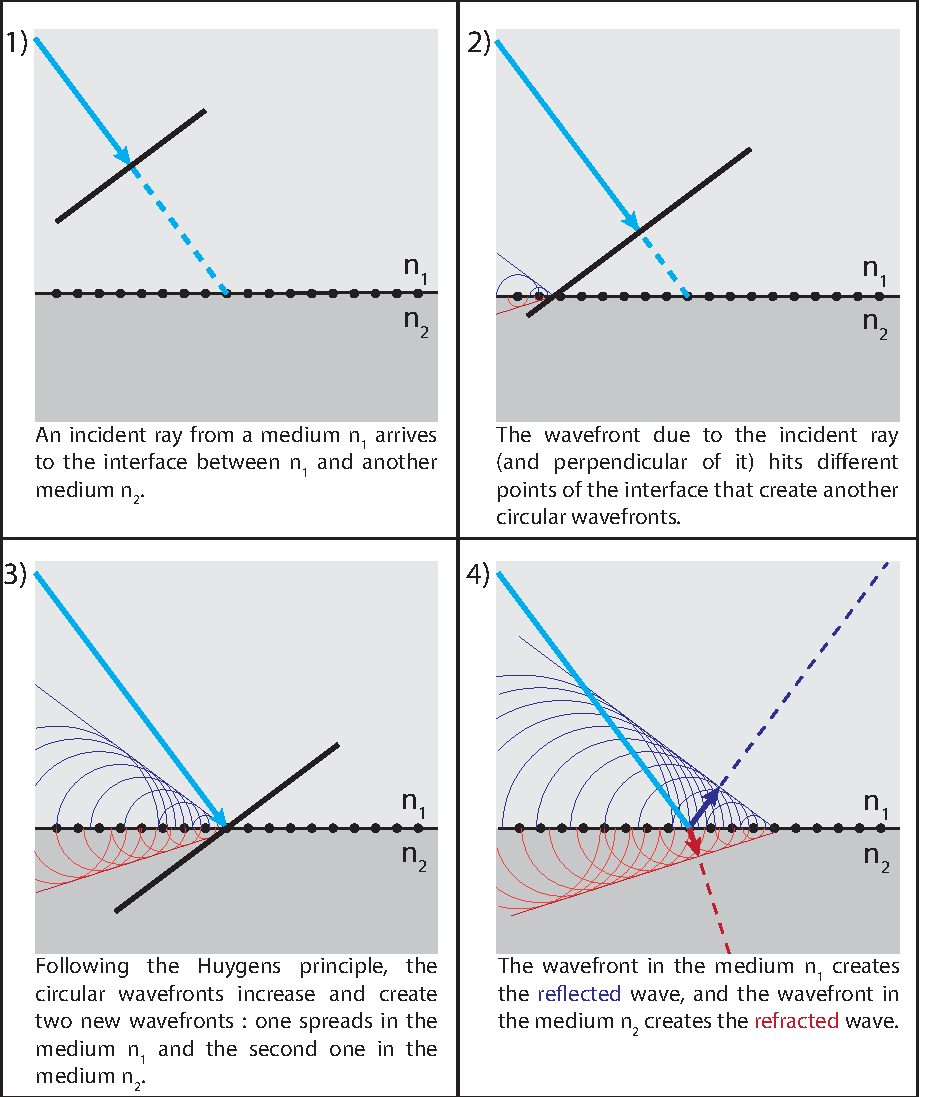
\includegraphics[trim = 0mm 100mm 30mm 0mm, clip,scale=0.7]{seismology/figures/huygens_explanation.pdf}
    \caption{Illustration of Huygens' principle. This phenomenon explains the creation of the reflected and refracted waves.}
    \label{figure_huygens_refracted_reflection}
\end{figure}
In optics, this principle allows to explain another complex phenomenon as the
diffraction .  At all times, the ray paths are normal to the wavefront
(Figure~\ref{fig:wr}).  As the wavefronts interact with boundaries between
differing velocity and/or acoustic impedance the wavefronts can reflect,
refract, and diffract.
\begin{figure}[hbtp]
    \centering
    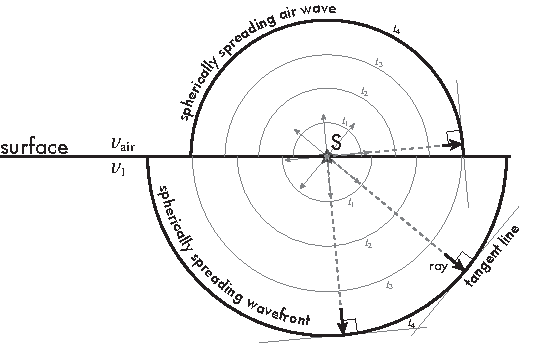
\includegraphics[]{seismology/figures/wavefronts&rays.pdf}
    \caption{Spherically spreading waves.  Rays paths are at right angles to the wavefront at all times.  What must be the relationship between the velocity of the wave in air versus the ground in this example?  Why?}
    \label{fig:wr}
\end{figure}

We will define the travel-time, $t$, as the minimum time that it takes a ray to
travel from a source, S, to any point, R, by
\begin{equation}
    t = \min \int_{\mathrm{S}}^{\mathrm{R}} \frac{\dd{\ell}}{v(x,y,z)},
\end{equation}
where $v$ is the velocity of the medium and $\dd{\ell}$ is the infinitesimal
length along the ray path.  The travel-time relationship is called Fermat's
principle.  In general the points that we care about are the receiver locations,
$\mathrm{R}_{n}$.

\subsection{Direct waves}
At some distance from the source, we place a receiver (R).  There are two waves
that directly travel from the source to the receiver, an {\bf air wave} which
travels just above the ground surface and a {\bf direct wave} which travels just
below the surface (Figure~\ref{fig:exwaves}).  There are also surface waves
(Love and Raleigh) which travel directly from the source to the receiver
(a.k.a.\ {\bf ground roll}), but they are not properly described by the ray
theory.  In general surface waves are a noise source for the types of
experiments that we are discussing.
\begin{figure}[hbtp]
    \centering
    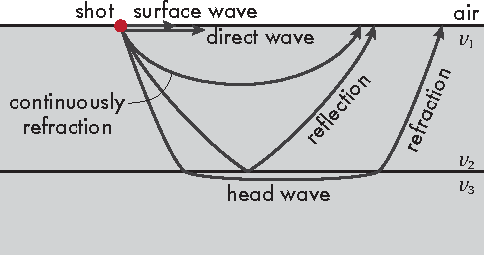
\includegraphics[]{seismology/figures/exploration_waves.pdf}
    \caption{Terminology of wave types emanating from an active source.}
    \label{fig:exwaves}
\end{figure}

For a direct wave, the travel-time between the source, S, and receiver, R,
separated by a distance, $d$, is
\begin{equation}
    t = \frac{\ell_{\mathrm{SR}}}{v_1} = \frac{d}{v_{1}},
\end{equation}
where $v_1$ is the constant velocity of the surface layer.


\subsection{Acoustic Impedance}
There are several types of indirect waves that are possible.  A ray travels
until it reaches an interface.  At the interface, some of the energy is
reflected and the remainder is transmitted.  The amount of energy that is
transmitted or reflected at a boundary is dependent upon the relative acoustic
impedance of the two layers.  We define the acoustic impedance of layer $j$ as,
$Z_j = \rho_j V_j$, where $\rho_j$ is the layer density and $V_j$ is the layer
velocity.  We can estimate the reflection coefficient, $R$, and transmission
coefficient, $T$, of a normally incident wave as
\begin{equation}
    R = \frac{Z_2 - Z_1}{Z_2 + Z_1} \mbox{ and }
    T = \frac{2 Z_1}{Z_2 + Z_1},
\end{equation}
respectively, where $R + T = 1$.  Note the similarity between these coefficients
and the complementary results from electromagnetic waves.  Since the reflection
coefficient depends upon the density as well as the velocity, a change in
velocity does not necessarily imply a reflection is guaranteed to occur.  Why
might the velocity decrease, but density increase? Or conversely, why density
decrease but velocity increase?


\subsection{Reflection}
Let us consider the constant velocity case where the ray strikes a horizontal
interface at an incident angle $\theta_i$ w.r.t.\ the vertical.  The wave is
reflected toward the surface at a reflection angle $\theta_i'$ w.r.t.\ the
vertical.  The ray travels from the source (S), bounces off an layer interface
at a point (B) a disstance $x$ from S, and is reflected to the surface and
measured at a receiver (R) a distance $d$ from S (Figure~\ref{fig:reflect}).
\begin{figure}[hbtp]
  \centerline{
    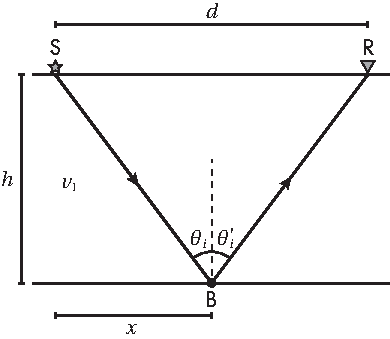
\includegraphics[]{seismology/figures/reflection.pdf}
  }
  \caption{Reflection of seismic waves.}
  \label{fig:reflect}
\end{figure}

We wish to find the minimum travel-time necessary for this path, which can be simply written as the sum of the travel-times from the source to the bounce point (SB) and the bounce point to the receiver (BR),
\begin{equation}
    t = \frac{\ell_{\mathrm{SB}}}{v_1} + \frac{\ell_{\mathrm{BR}}}{v_1} =
        v_1^{-1} \left[ (h^2 + x^2)^{1/2} + (h^2 + (d - x)^2)^{1/2} \right].
\end{equation}
To find the minimum, we take the derivative w.r.t.\ $x$ and set equal to zero,
\begin{equation}
    \dv{t}{x} = 0 = v_1^{-1}
        \left[ \frac{x}{(h^2 + x^2)^{1/2}} 
        - \frac{d - x}{(h^2 + (d - x)^2)^{1/2}} \right].
\end{equation}
Solving for $d$, we find
\begin{equation}
    d = 2 x,
\end{equation}
which implies that $\theta_i = \theta_i'$.

Hence we can write the travel-time for a reflected wave as
\begin{align}
    t(x) & = \frac{2}{v_1}
        \left[ h^2 + \left( \frac{x}{2} \right)^2 \right]^{1/2},\\
        & = \frac{2 h}{v_1}
        \left[ 1 + \left( \frac{x}{2 h} \right)^2 \right]^{1/2},
\end{align}
where $x$ is now the distance between the source and receiver.  The shape of this reflection travel-time function is a hyperbola with asymptotes at $t = \pm x v_1^{-1}$.

When the source and receiver are co-located ($x = 0$), the travel-time for a reflection is
\begin{equation}
    t_0 = \frac{2 h}{v_1}.
\end{equation}
This result allows us to write $t(x)$ in terms of $t_0$,
\begin{align}
    t(x) &= t_0 \left[ 1 + \left( \frac{x}{2 h} \right)^2 \right]^{1/2} \\
    &= t_0 \left[ 1 + \left( \frac{x}{t_0 v_1} \right)^2 \right]^{1/2},
\end{align}

\subsubsection{Normal Moveout}
Typically when we collect geophysical data, the data we collect can be modeled by physical principles.  However, we often do not know all or most of the physical parameters that result in the response that we observe.  For example, in the case above, we have derived a physical expression for the travel-time.  But our result is dependent upon the unknown parameters for the thickness of the layer and its velocity.  For the case of reflections, a method called {\bf normal moveout} is employed and whos description is given below.

Let us define a parameter called the normal moveout $t_{\mathrm{NMO}}(x) = t(x) - t_0$,
\begin{equation}
    t_{\mathrm{NMO}} = t_0 \left[ 1 + \left( \frac{x}{2 h} \right)^2 \right]^{1/2} - t_0.
\end{equation}
If we collect our data such that our geophones are close to the source w.r.t.  the depth of the layer ($x \ll h$), we can use a Taylor series expansion to write
\begin{equation*}
    t_{\mathrm{NMO}} = t_0 \left[ 1 + \frac{1}{2}\left( \frac{x}{2 h} \right)^2
    + \cdots \right] - t_0,
\end{equation*}
Ignoring terms higher than $x^2$, we find
\begin{align}
    t_{\mathrm{NMO}} & = \frac{1}{2}\left( \frac{x}{2 h} \right)^2, \\
        & = \frac{x^2}{2 v_1^2 t_0}. \\
\end{align}

We have now derived an expression for the normal moveout with respect to only one unknown, the velocity.  Once we solve for the velocity, we can then solve for the layer thickness using the expression for $t_0$.


\subsection{Refraction}
Refraction refers to the bending of a wave at a boundary due to a contrast in physical properties.  In our case, the physical property that results in bending the waves is the velocity of the medium.

Let us consider, as before, the constant velocity case where the ray strikes a horizontal interface at an incident angle $\theta_i$ w.r.t.\ the vertical (Figure~\ref{fig:refract}).  The wave is transmitted through the lower medium, but is refracted by an angle $\theta_r$ w.r.t.\ the vertical.  The ray travels from the source (S), bends at the layer interface at a point (B), and is measured at a point (R) a horizontal distance $d$ from the source.
\begin{figure}[hbtp]
  \centerline{
    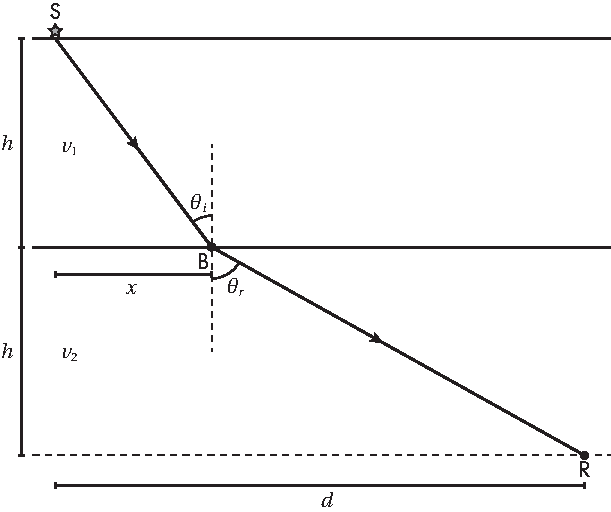
\includegraphics[]{seismology/figures/refraction.pdf}
  }
  \caption{Refraction of seismic waves.}
  \label{fig:refract}
\end{figure}

The travel-time from S to R may be written as the sum of the travel-times from
SB and BR,
\begin{equation}
    t = \frac{\ell_{\mathrm{SB}}}{v_1} + \frac{\ell_{\mathrm{BR}}}{v_2} =
        \frac{(h^2 + x^2)^{1/2}}{v_1} + \frac{(h^2 + (d - x)^2)^{1/2}}{v_2} .
\end{equation}
To find the minimum, we take the derivative w.r.t.\ $x$ and set equal to zero,
\begin{equation}
    \dv{t}{x} = 0 = 
        v_1^{-1}\frac{x}{(h^2 + x^2)^{1/2}} 
        - v_2^{-1}\frac{d - x}{(h^2 + (d - x)^2)^{1/2}} .
\end{equation}
We can use the trigonometric relations to rewrite the above result as
\begin{equation}
    \frac{\sin \theta_i}{v_1} = \frac{\sin \theta_r}{v_2}.
\end{equation}
This relation is known as Snell's Law.  Unlike reflection where reflections only occur at interfaces with differing impedance, not simply differing velocity, refractions occur when the velocities differ at an interface.

If the velocities are such that $v_2 > v_1$, then the ray is bent toward the interface, $\theta_r > \theta_i$.  There exists a critical incidence angle, $\theta_c$, such that the wave is refracted parallel to the layer interface, i.e.\ critically refracted (Figure~\ref{fig:cr}).  The critical angle occurs when $\theta_r = \frac{\pi}{2} = 90^\circ$.  This allows us to solve for the critical angle in terms of the velocity ratio
\begin{equation}
    \sin \theta_c = \frac{v_{1}}{v_2}.
\end{equation}
\begin{figure}[hbtp]
    \centering
    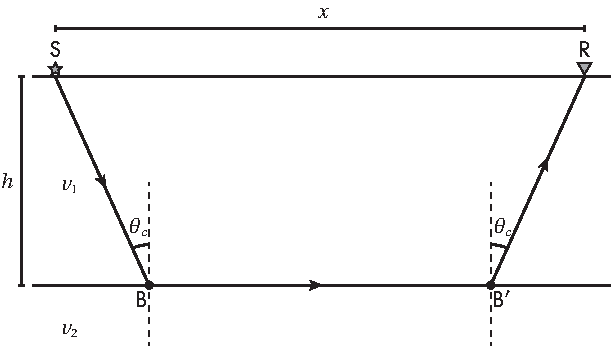
\includegraphics[]{seismology/figures/critical_refraction.pdf}
    \caption{Critical angle and double refraction of seismic waves.}
    \label{fig:cr}
\end{figure}

Critically refracted waves are important as they continuously refract back up into the layer above and return to the surface.  The travel-time for a refracted wave between the source, S, and a receiver, R, can be found by tracing a ray from the source at an angle critical to the interface, along the interface, and from the interface to the receiver at the critical angle,
\begin{equation}
    t = \frac{\ell_\mathrm{SB}}{v_1} + \frac{\ell_\mathrm{BB'}}{v_2} +
    \frac{\ell_\mathrm{B'R}}{v_1}.
\end{equation}
For a horizontal layer, the lengths SB and B'R are equal.  The resulting
travel-time is
\begin{equation}
    t = 2 \frac{h}{v_1 \cos \theta_c} + \frac{x - 2 h \tan \theta_c}{v_2}.
\end{equation}
We can simplify the above result somewhat by rearranging terms
\begin{align*}
    t & = \frac{x}{v_2} + 2 h
        \left( \frac{1}{v_1 \cos \theta_c}
        - \frac{\sin \theta_c}{v_2 \cos \theta_c} \right), \\
    & = \frac{x}{v_2} + 2 h
        \left( \frac{v_2 - v_1 \sin \theta_c}{v_1 v_2 \cos \theta_c} 
         \right),
\end{align*}
at this point we can use Snell's Law ($\sin \theta_c = \frac{v_1}{v_2}$),
\begin{align*}
    t & = \frac{x}{v_2} + 2 h
        \left( \frac{v_2 - v_2 \sin^2 \theta_c}{v_1 v_2 \cos \theta_c} \right), \\
    & = \frac{x}{v_2} + 2 h
        \left( \frac{1 - \sin^2 \theta_c}{v_1 \cos \theta_c} \right),
\end{align*}
recalling $\cos^2 \theta + \sin^2 \theta \equiv 1$, we arrive at
\begin{equation}
    t = \frac{x}{v_2} +
        \frac{2 h \cos \theta_c}{v_1} .
\end{equation}
If we wish, we may remove the dependence upon $\theta_c$ and write the result in terms of the velocities as
\begin{align}
    t & = \frac{x}{v_2} +
        \frac{2 h (v_2^2 - v_1^2)^{1/2}}{v_1 v_2} , \\
      & = \frac{x}{v_2} +
      2 h \left( \frac{1}{v_1^2} - \frac{1}{v_2^2} \right)^{1/2}.
\end{align}

The resulting travel-time for a doubly refracted wave is the equation of a line (i.e.\ $t = m x + t_i$) with the slope $m = \frac{1}{v_1}$, and intercept time
\begin{align}
    t_i = \frac{2 h (v_2^2 - v_1^2)^{1/2}}{v_1 v_2} .
\end{align}

While reflections occur whenever there is an acoustic impedance, a refracted wave only occurs when $\theta = \theta_c$.  Hence, at receiver locations within a given proximity of source, a refracted wave cannot physically appear.  If $v_1 > v_2$ then the ray is bent away from the interface, $\theta_i > \theta_r$.  As a result, the waves cannot be critically refracted and will not return to the surface.  While refractions can still occur from deeper layers, the effect of a low velocity layer beneath a higher velocity is hidden and results in a larger predicted thickness of the layer below the low velocity zone.

%\subsection{Tomography}
%So far, we have only described seismic waves traveling through layered media, 

\nocite{Grant&West1965}

\bibliographystyle{elsarticle-harv}
\bibliography{ref}
